%\documentclass[first,firstsupp,handout,compress,notes,navigation]{ETHclass} 
%\documentclass[first,firstsupp,handout,notes]{ETHclass} 
%\documentclass[first,firstsupp,handout]{ETHclass} 
%\documentclass[first,firstsupp,notes]{ETHclass} 
\documentclass[first,firstsupp]{ETHclass}
\usepackage{etex}
\usepackage{siunitx}
\usepackage{textcomp}
\usepackage{booktabs}
\usepackage{subcaption}

% Options for beamer:
%
% 9,10,11,12,13,14,17pt  Fontsizes
% 
% compress: navigation bar becomes smaller
% t       : place contents of frames on top (alternative: b,c)
% handout : handoutversion
% notes   : show notes
% notes=onlyslideswithnotes
%
%hyperref={bookmarksopen,bookmarksnumbered} : Needed for menues in
%                                             acrobat. Also need
%                                             pdftex as option or 
%                                             compile with
% pdflatex '\PassOptionsToPackage{pdftex,bookmarksopen,bookmarksnumbered}{hyperref} \input{file}'

%\usepackage{beamerseminar}
%\usepackage[accumulated]{beamerseminar}
                                % remove ``accumulated'' option
                                % for original behaviour
\usepackage{beamerbasenotes}
%\setbeamertemplate{note page}[plain] 
%\setbeameroption{notes on second screen}


\usepackage[pdf]{pstricks}


%\setbeamertemplate{note page}[plain] 
\setbeamertemplate{note page}{\ \\[.3cm]
    \textbf{\color{blue}Notes:}\\%[0.1cm]
    {\footnotesize %\tiny
    \insertnote}}
%\setbeameroption{notes on second screen}

    \usepackage{multimedia}

    \setbeamertemplate{navigation symbols}{} % suppresses all navigation symbols:
% \setbeamertemplate{navigation symbols}[horizontal] % Organizes the navigation symbols horizontally.
% \setbeamertemplate{navigation symbols}[vertical] % Organizes the navigation symbols vertically.
% \setbeamertemplate{navigation symbols}[only frame symbol] % Shows only the navigational symbol for navigating frames.

    \setlayoutscale{0.5}
    \setparametertextfont{\scriptsize}
    \setlabelfont{\scriptsize}

    \DeclareSIUnit[number-unit-product = \,]{\permille}{\textperthousand}
    \newcommand{\energy}{\mathcal{E}}
    \newcommand{\vcenteredinclude}[2]{\begingroup
        \setbox0=\hbox{\includegraphics[#1]{#2}}%
        \parbox{\wd0}{\box0}\endgroup}

        \begin{document}

        \title[First progress report]{Towards high-energy phase contrast imaging}
        \author{\emph{Matteo Abis}\inst{a} \and %
        Thomas Th\"uring\inst{a} \and %
        Marco Stampanoni\inst{a}}
        \institute[ETHZ and PSI]{\inst{a} ETH Z\"urich and Paul Scherrer
    Institut}
    \renewcommand{\today}{15th January 2013}
    \begin{frame}
        \maketitle
    \end{frame}
%\note{}

    \begin{frame}
        \frametitle{Why high energy?}
        $n = 1 - {\color{red}\delta} - i {\color{blue}\beta}$
        \begin{columns}
            \begin{column}
                {.85\textwidth}
                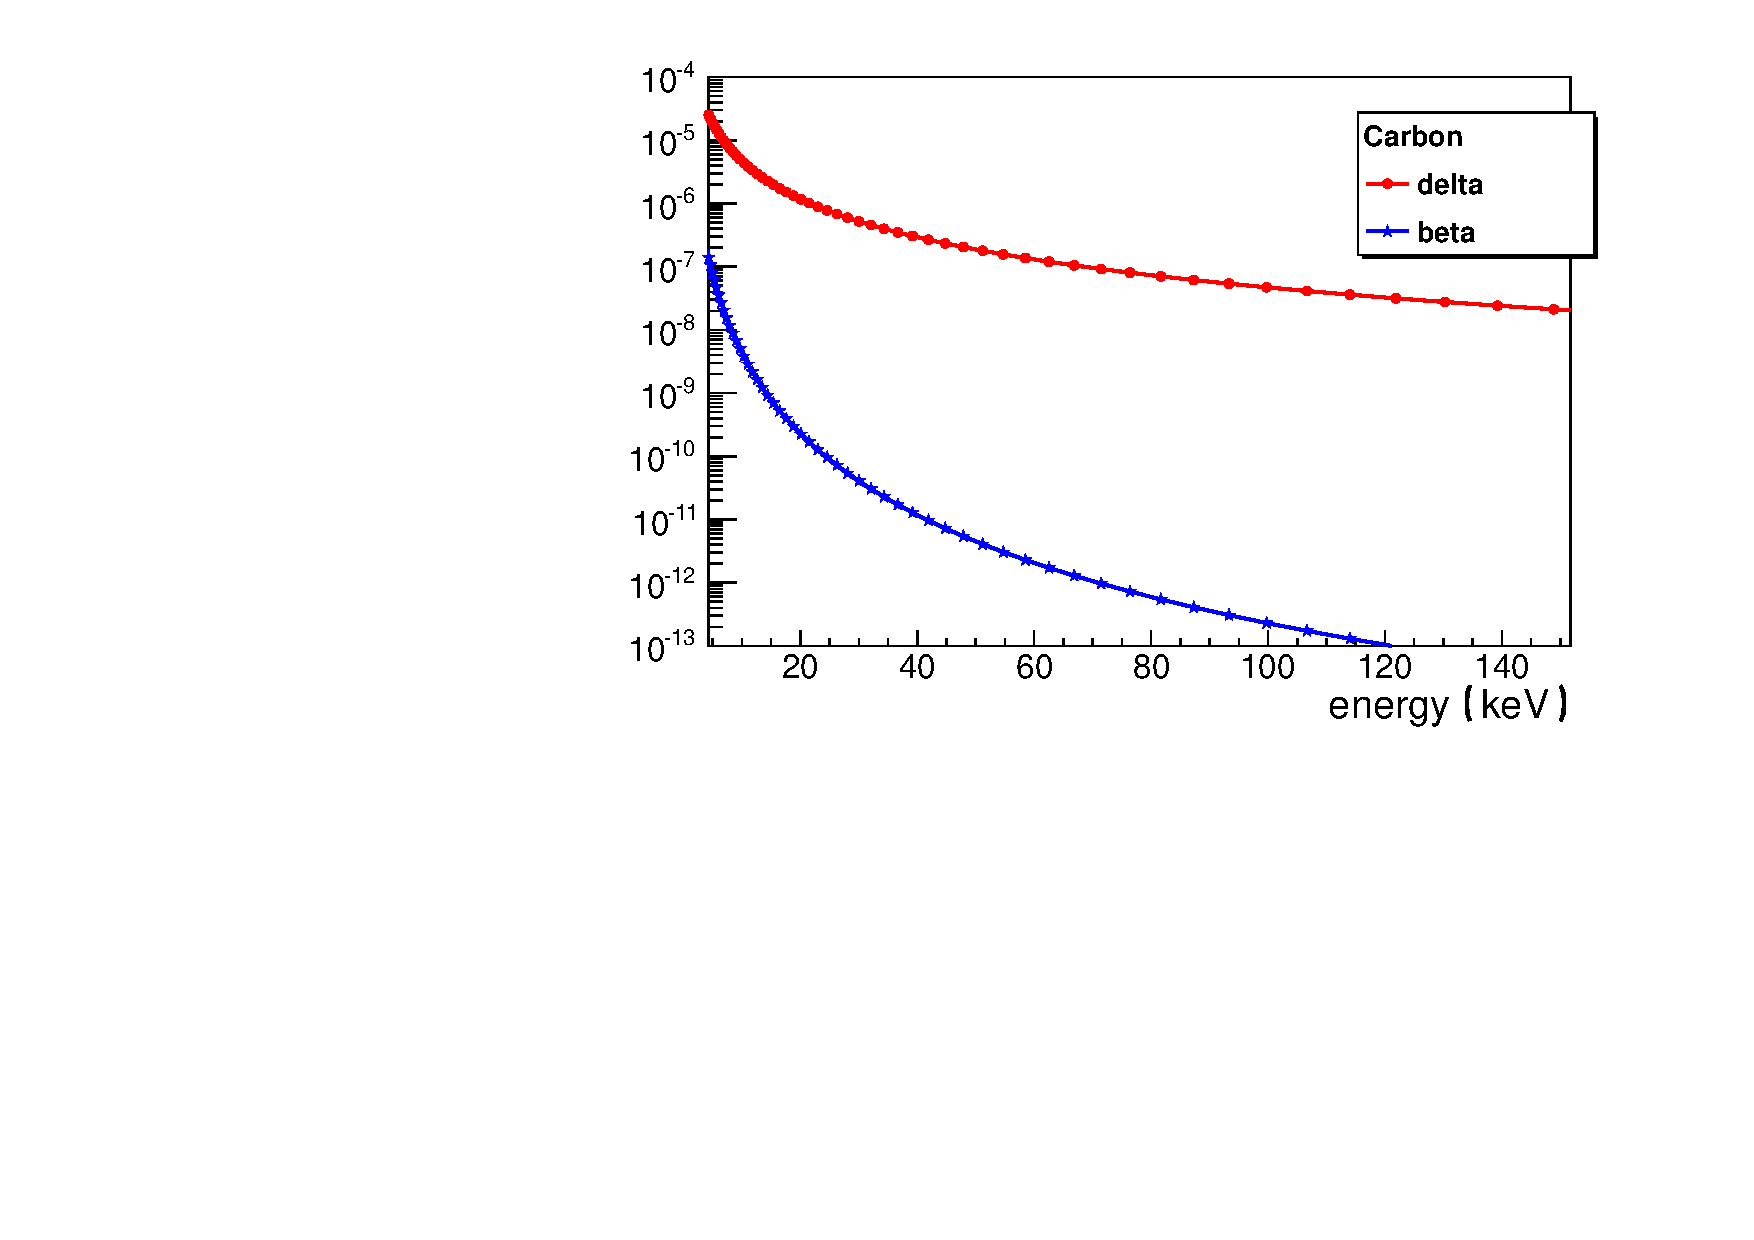
\includegraphics[width=.9\textwidth]{delta_beta_refraction_index_6_1_200}
            \end{column}
            \begin{column}
                {.15\textwidth}
                \begin{align*}
                    {\color{red}\delta} &{\color{red}\sim \energy^{-2}}\\
                    {\color{blue}\beta} &{\color{blue}\sim \energy^{-4}}
                \end{align*}
            \end{column}
        \end{columns}
        \begin{figure}[h]
            \centering
        \end{figure}
        good phase contrast with reduced dose.
    \end{frame}

    \begin{frame}
        \frametitle{What energy is \emph{high} energy?}
        Three mean energies
        \begin{itemize}
            \item \SI{60}{\kilo\electronvolt}
            \item \SI{100}{\kilo\electronvolt}
            \item \SI{120}{\kilo\electronvolt}
        \end{itemize}
        conventional tube $\rightarrow$ large bandwidth $\sim \SI{25}{\kilo\electronvolt}$
    \end{frame}

    \begin{frame}
        \frametitle{Seven different geometries}
        calculations and design: Thomas\textcopyright
        \begin{table}
            \centering
            \begin{tabular}{ccc}
                \toprule
                energy (\si{\kilo\electronvolt}) & total length (\si{\centi\metre}) & talbot order \\
                \midrule
                60  & 28  & 1\\
                60  & 66  & 3\\
                60  & 123 & 5\\
                100 & 40  & 1\\
                100 & 60 & 1\\
                100 & 123 & 3\\
                120 & 66 & 1\\
                \bottomrule
            \end{tabular}
        \end{table}
        \tiny{talbot $= p^2 / 8\lambda$}
    \end{frame}

    \begin{frame}
        \frametitle{The experimental setup}
        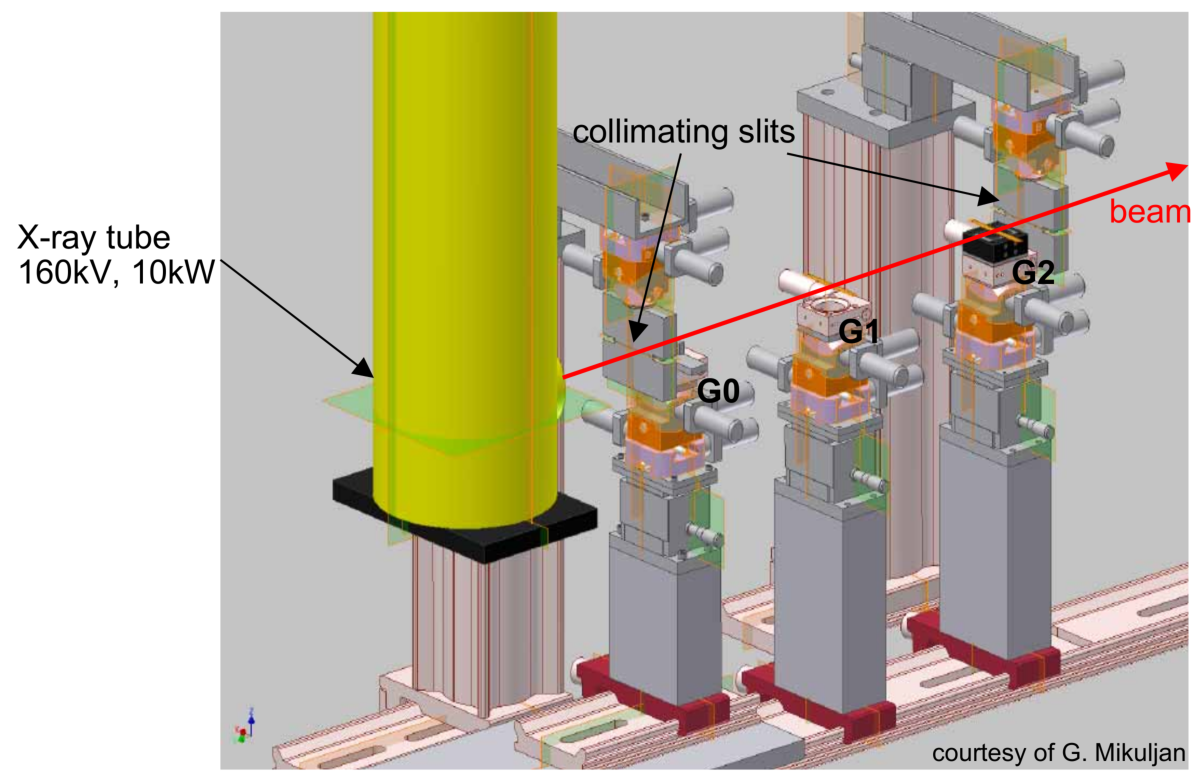
\includegraphics[width=.9\textwidth]{experimental_setup}
    \end{frame}

    \begin{frame}
        \frametitle{The Gotthard detector}
        \begin{columns}
            \begin{column}
                {0.45\textwidth}
                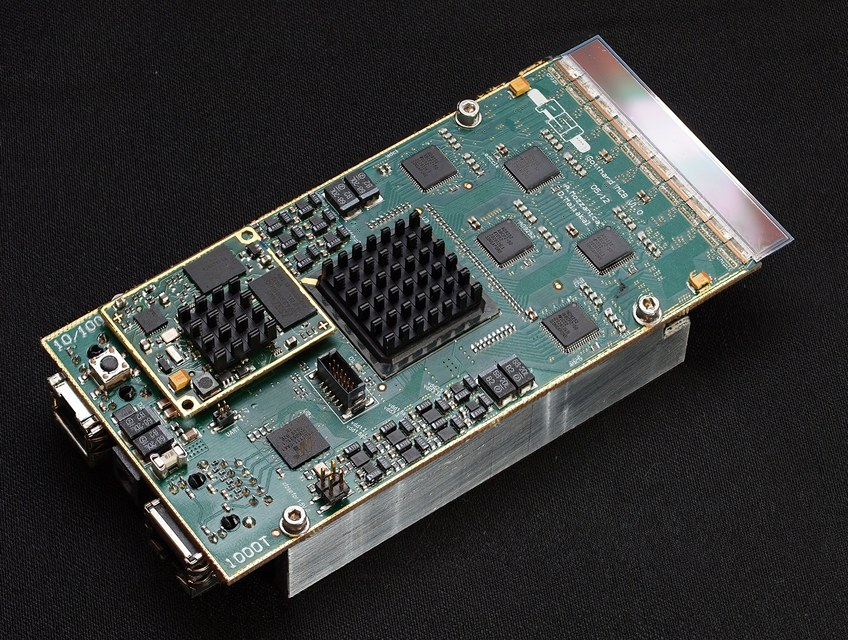
\includegraphics[width=\textwidth]{gotthard}
            \end{column}
            \begin{column}
                {0.45\textwidth}
                \begin{itemize}
                    \item silicon strips
                    \item photon counting
                    \item pitch \SI{50}{\micro\metre}
                    \item depth \SI{8}{\milli\metre}
                    \item thickness \SI{320}{\micro\metre}
                    \item linearity (energy) $< \SI{0.5}{\percent}$
                \end{itemize}
            \end{column}
        \end{columns}
    \end{frame}

    \begin{frame}
        \frametitle{The gratings}
        The biggest challenge:
        \begin{itemize}
            \item fan geometry $\rightarrow$ bent gratings
            \item pitch $= \SI{2.8}{\micro\metre}$
            \item thickness $= \SI{800}{\micro\metre}$
        \end{itemize}
        Very high aspect ratio $\rightarrow$ edge-on illumination\\
        \begin{figure}[h]
            \centering
            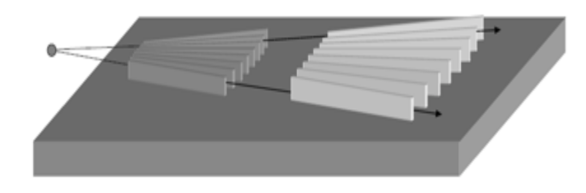
\includegraphics[height=.20\textheight]{edgeon}
        \end{figure}
        \tiny{(EP10167569 by M. Stampanoni and C. David)}
    \end{frame}

    \begin{frame}
        \frametitle{Edge-on illumination}
        \begin{itemize}
            \item arbitrary aspect ratio is possible
            \item difficult alignment (no Moir\'e pattern)
            \item 1D projections
            \item 2D with tomographic scans
            \item sample on a rotation stage
        \end{itemize}
    \end{frame}

    \begin{frame}
        \frametitle{The gratings: electron microscope pictures}
        delivered on 10th December from \vcenteredinclude{width=3cm}{microworks}
        \begin{table}
            \centering
            \begin{tabular}{cc}
                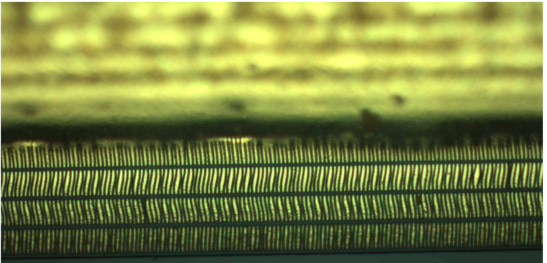
\includegraphics[width=.45\textwidth]{sem3} & 
                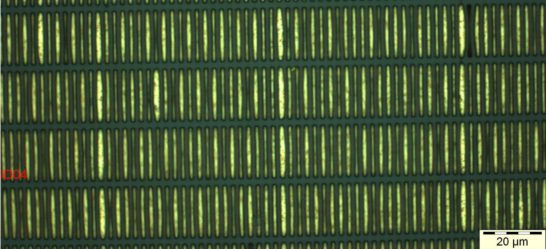
\includegraphics[width=.45\textwidth]{sem1}\\
                & 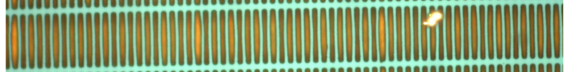
\includegraphics[width=.45\textwidth]{sem2}
            \end{tabular}
        \end{table}
    \end{frame}

    \begin{frame}
        \frametitle{The gratings: TOMCAT images}
        \begin{table}
            \centering
            \begin{tabular}{cc}
                \multicolumn{2}{c}{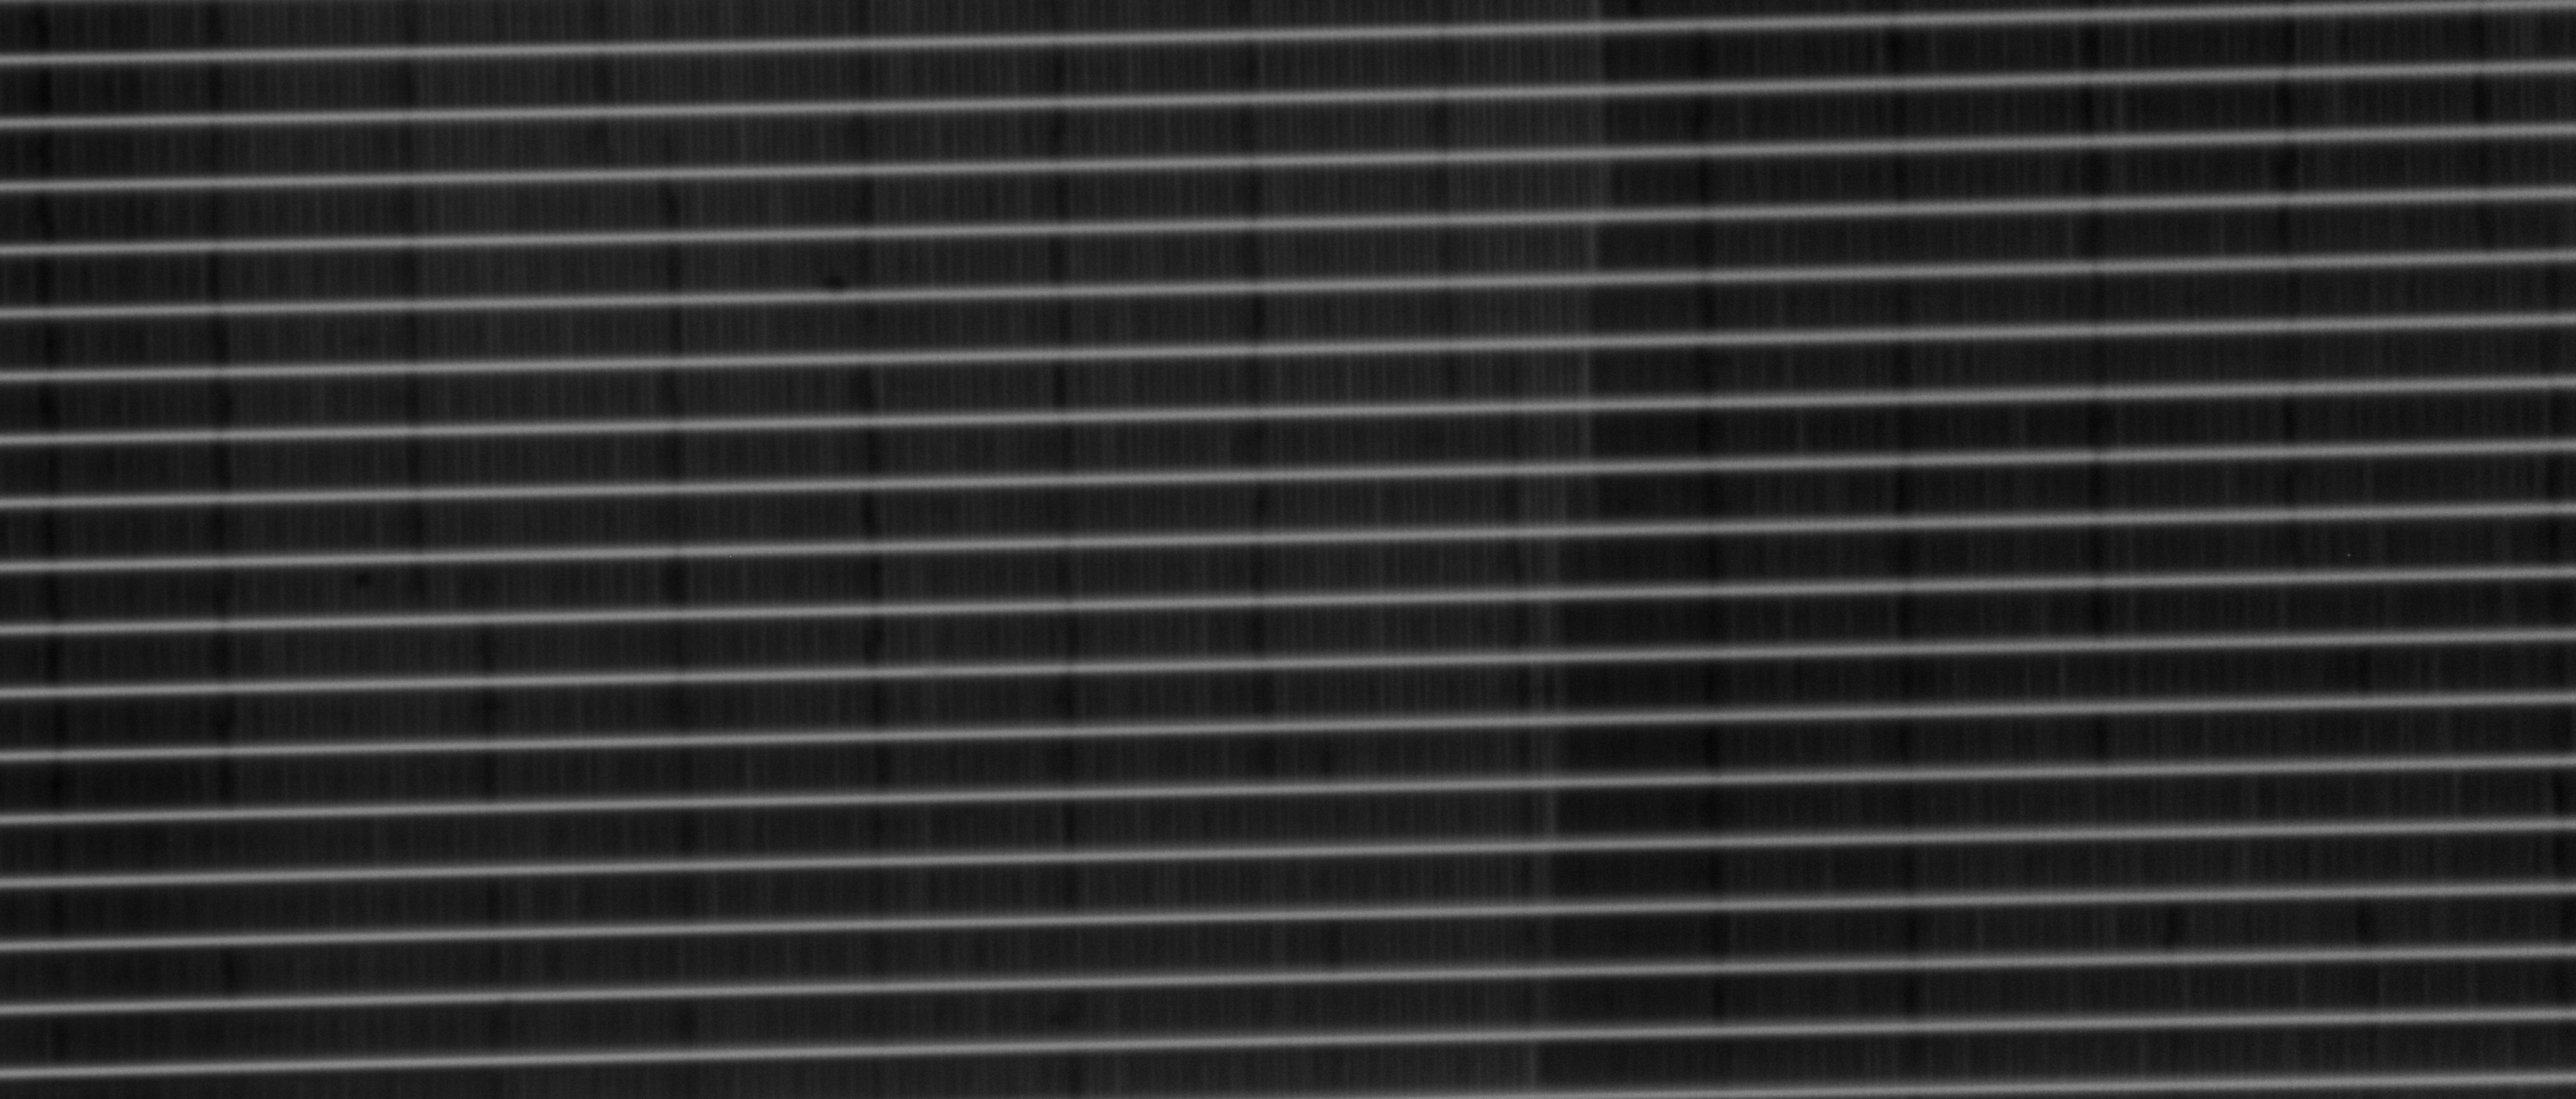
\includegraphics[width=.7\textwidth]{tomcat3}}
                \\
                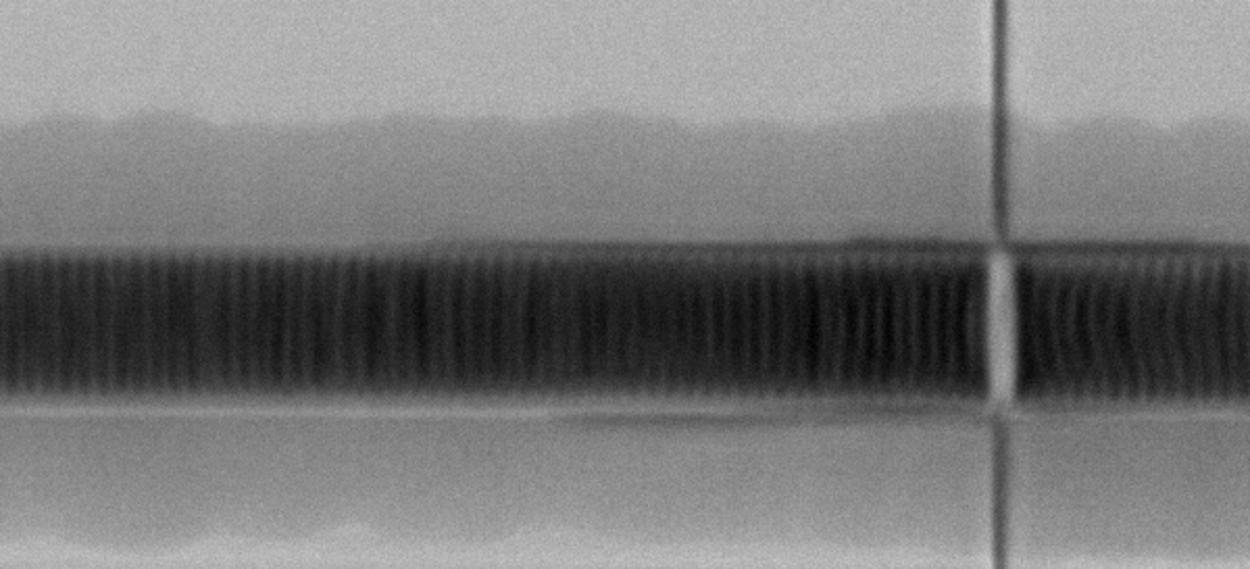
\includegraphics[width=.35\textwidth]{tomcat1} & 
                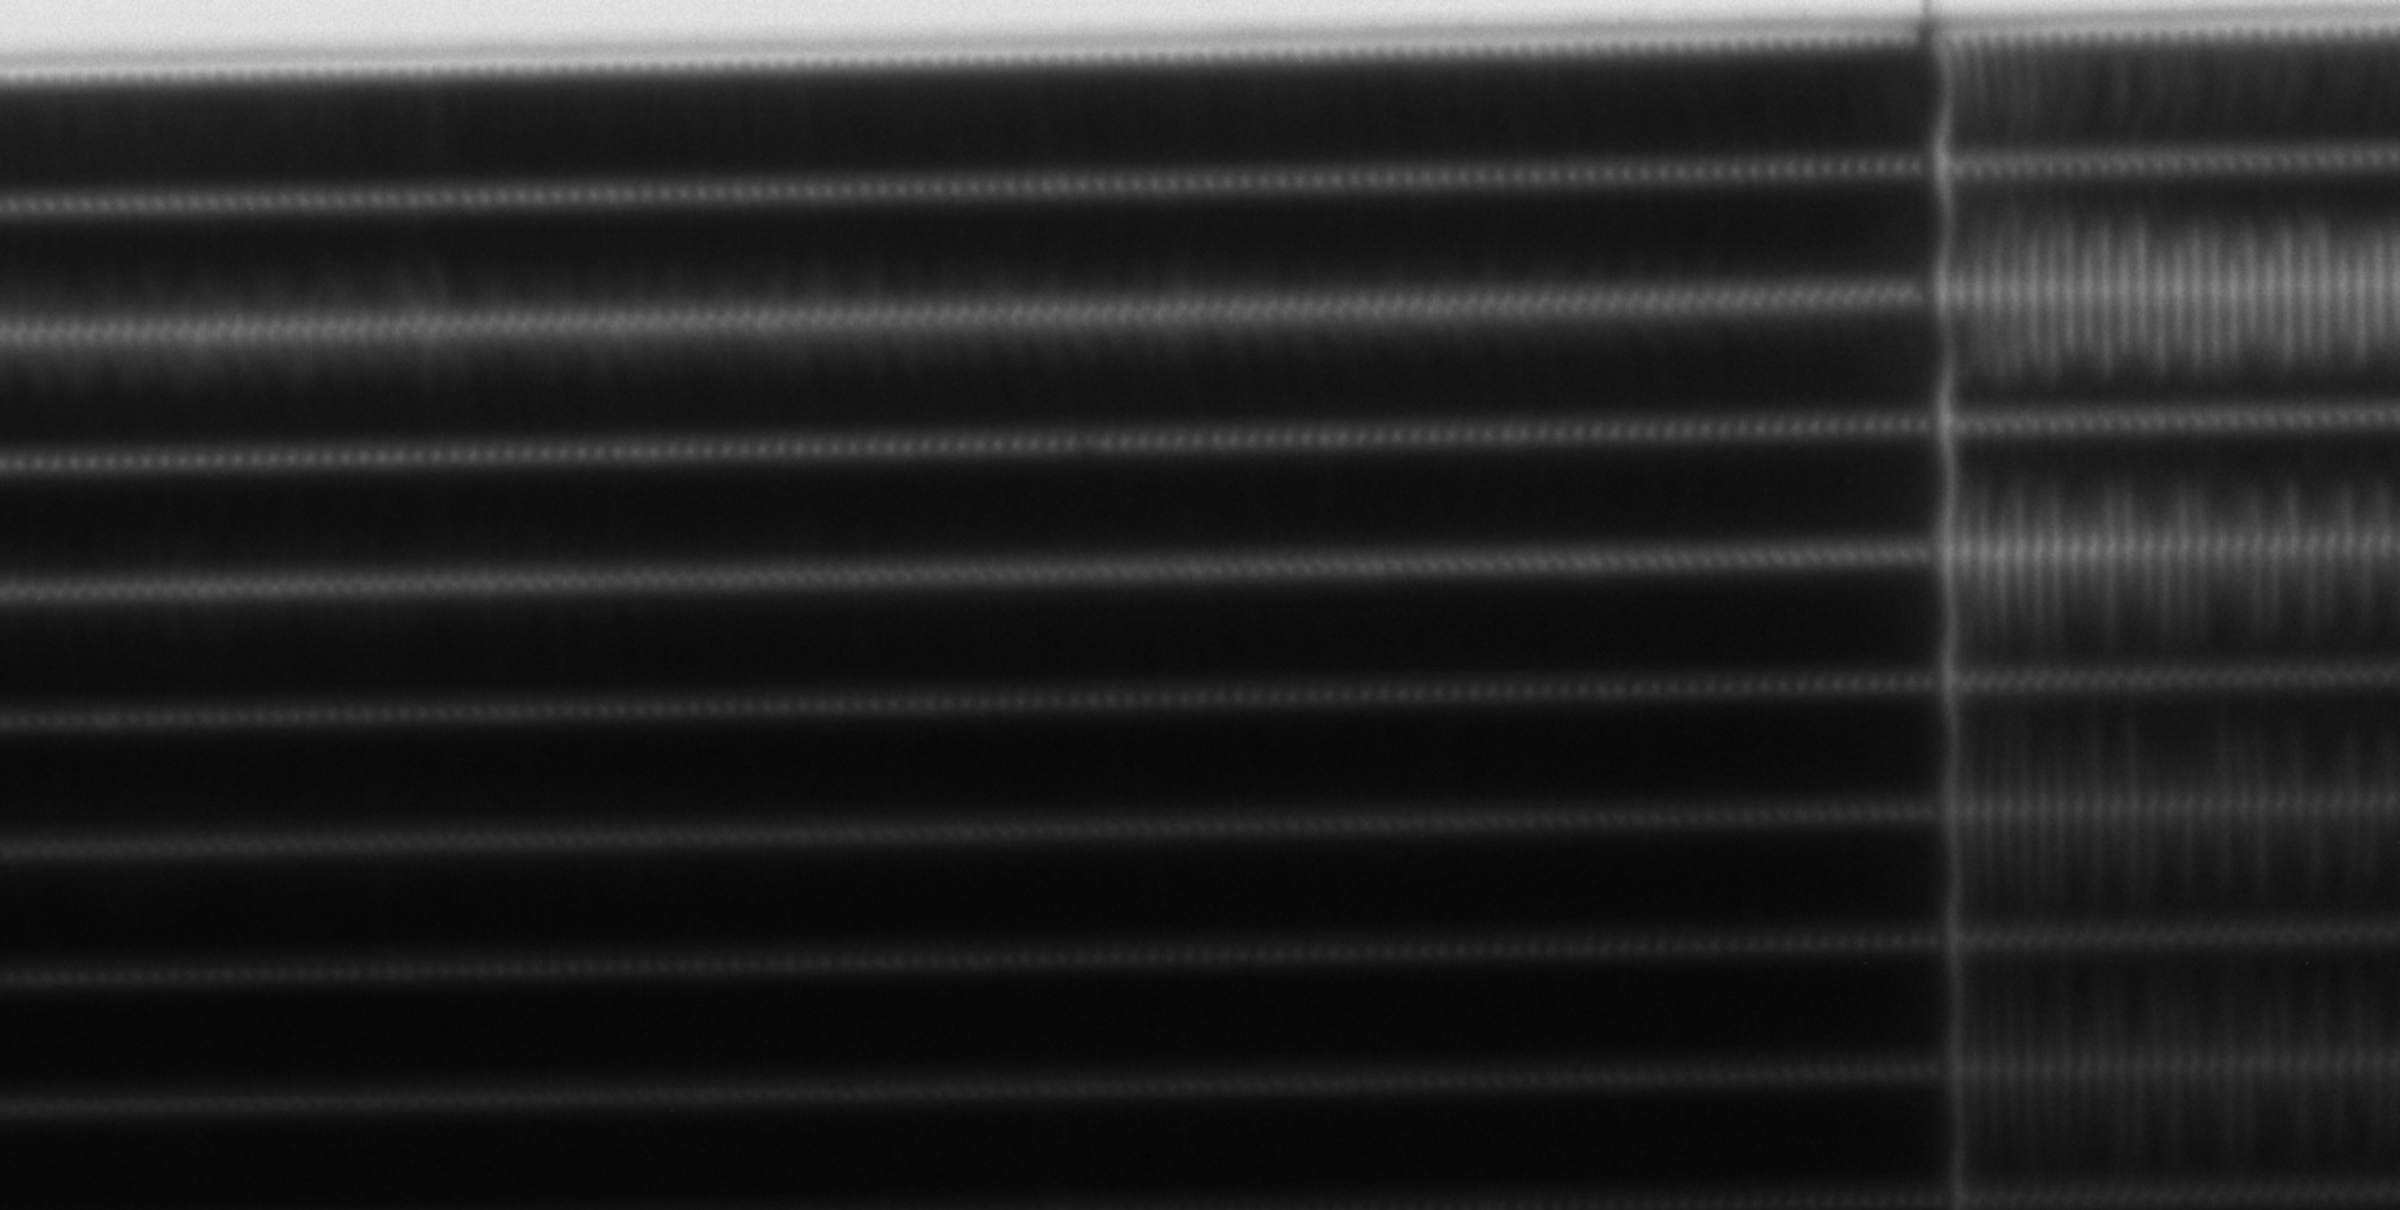
\includegraphics[width=.35\textwidth]{tomcat2}
            \end{tabular}
        \end{table}
    \end{frame}

    \begin{frame}
        \frametitle{Grating defects}
        \begin{itemize}
            \item overgrowth
            \item nonparallel and distorted grooves
            \item secondary structures
        \end{itemize}
    \end{frame}

    \begin{frame}
        \frametitle{X-ray filters}
        example: at \SI{60}{\kilo\electronvolt} useful window
        \SIrange{50}{75}{\kilo\electronvolt}
        \begin{figure}[h]
            \centering
            \begin{subfigure}
                [h]{.49\textwidth}
                \centering
                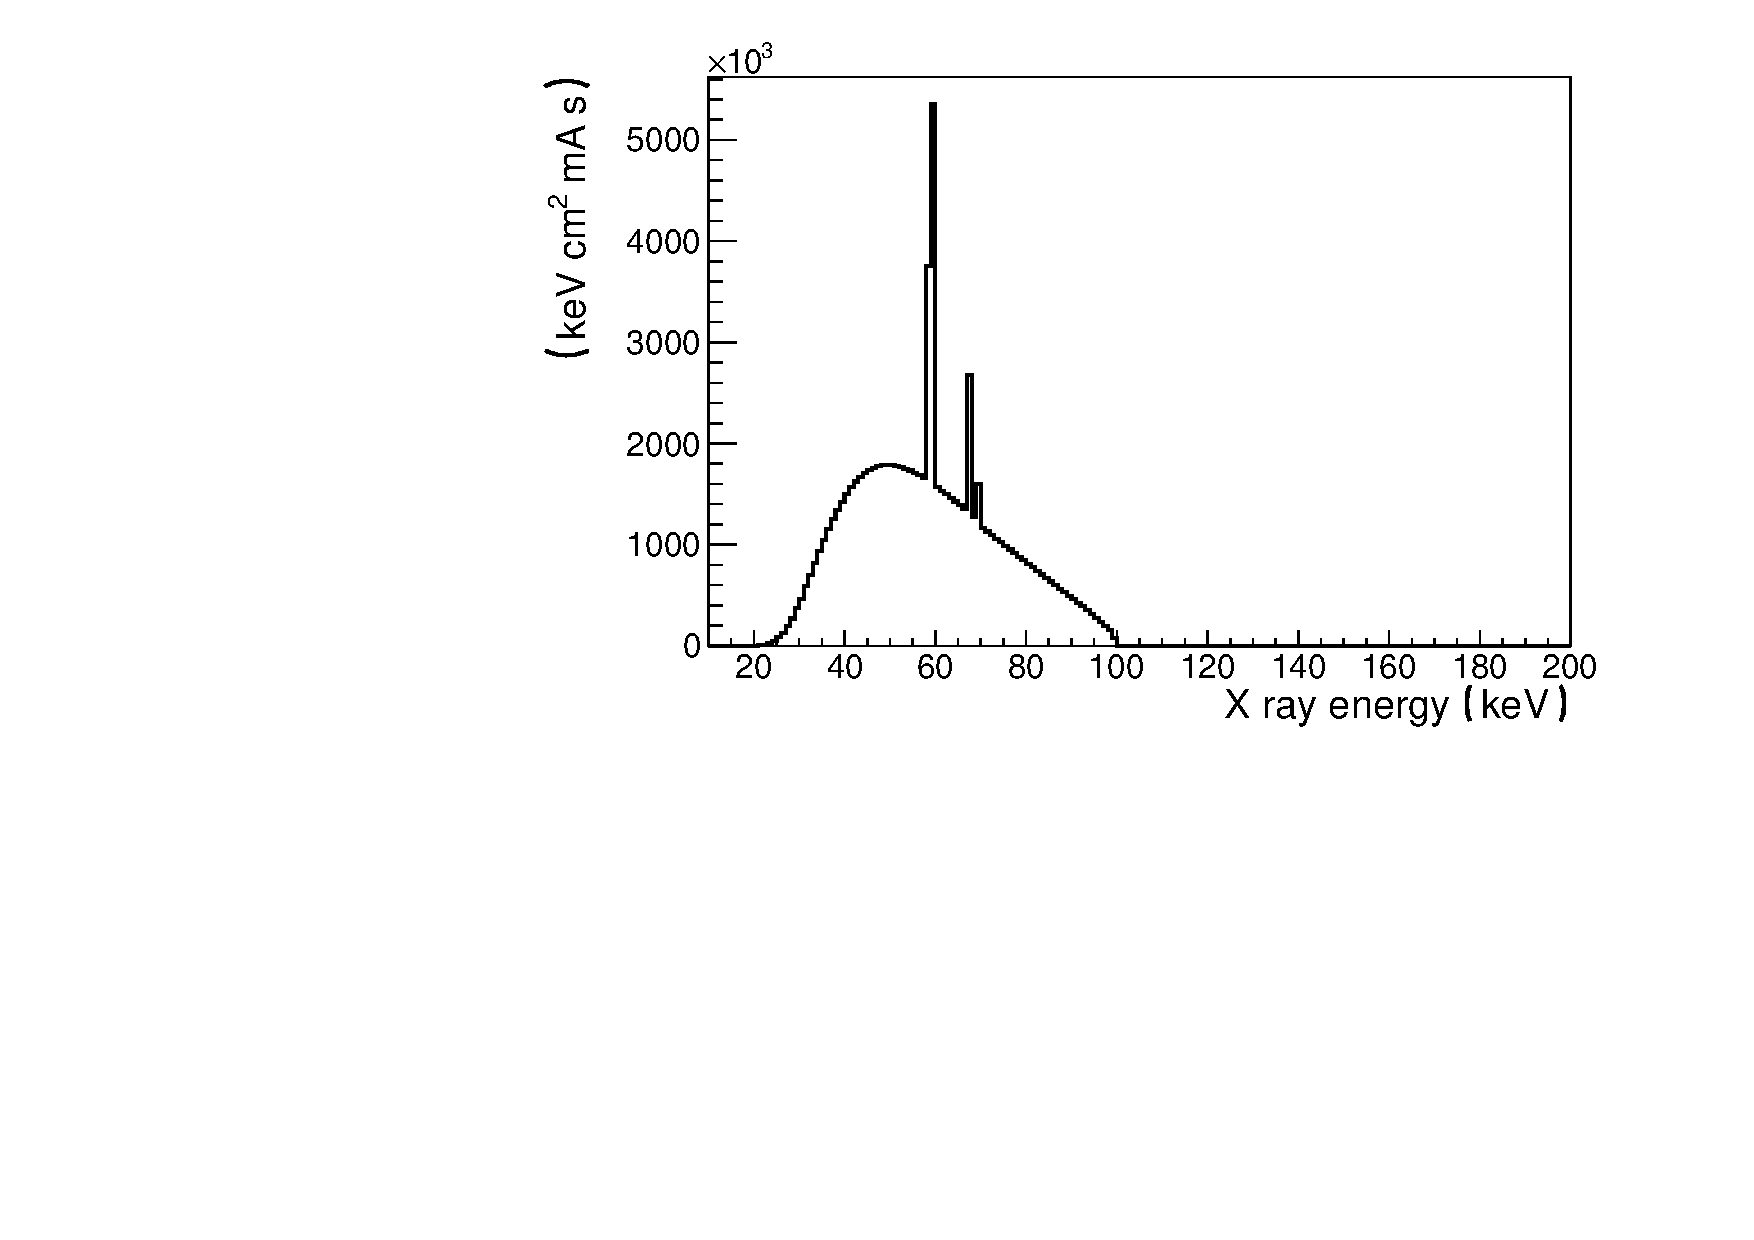
\includegraphics[width=\textwidth]{unfiltered_spectrum} 
                \caption*{tube spectrum}
            \end{subfigure}
            \begin{subfigure}
                [h]{.49\textwidth}
                \centering
                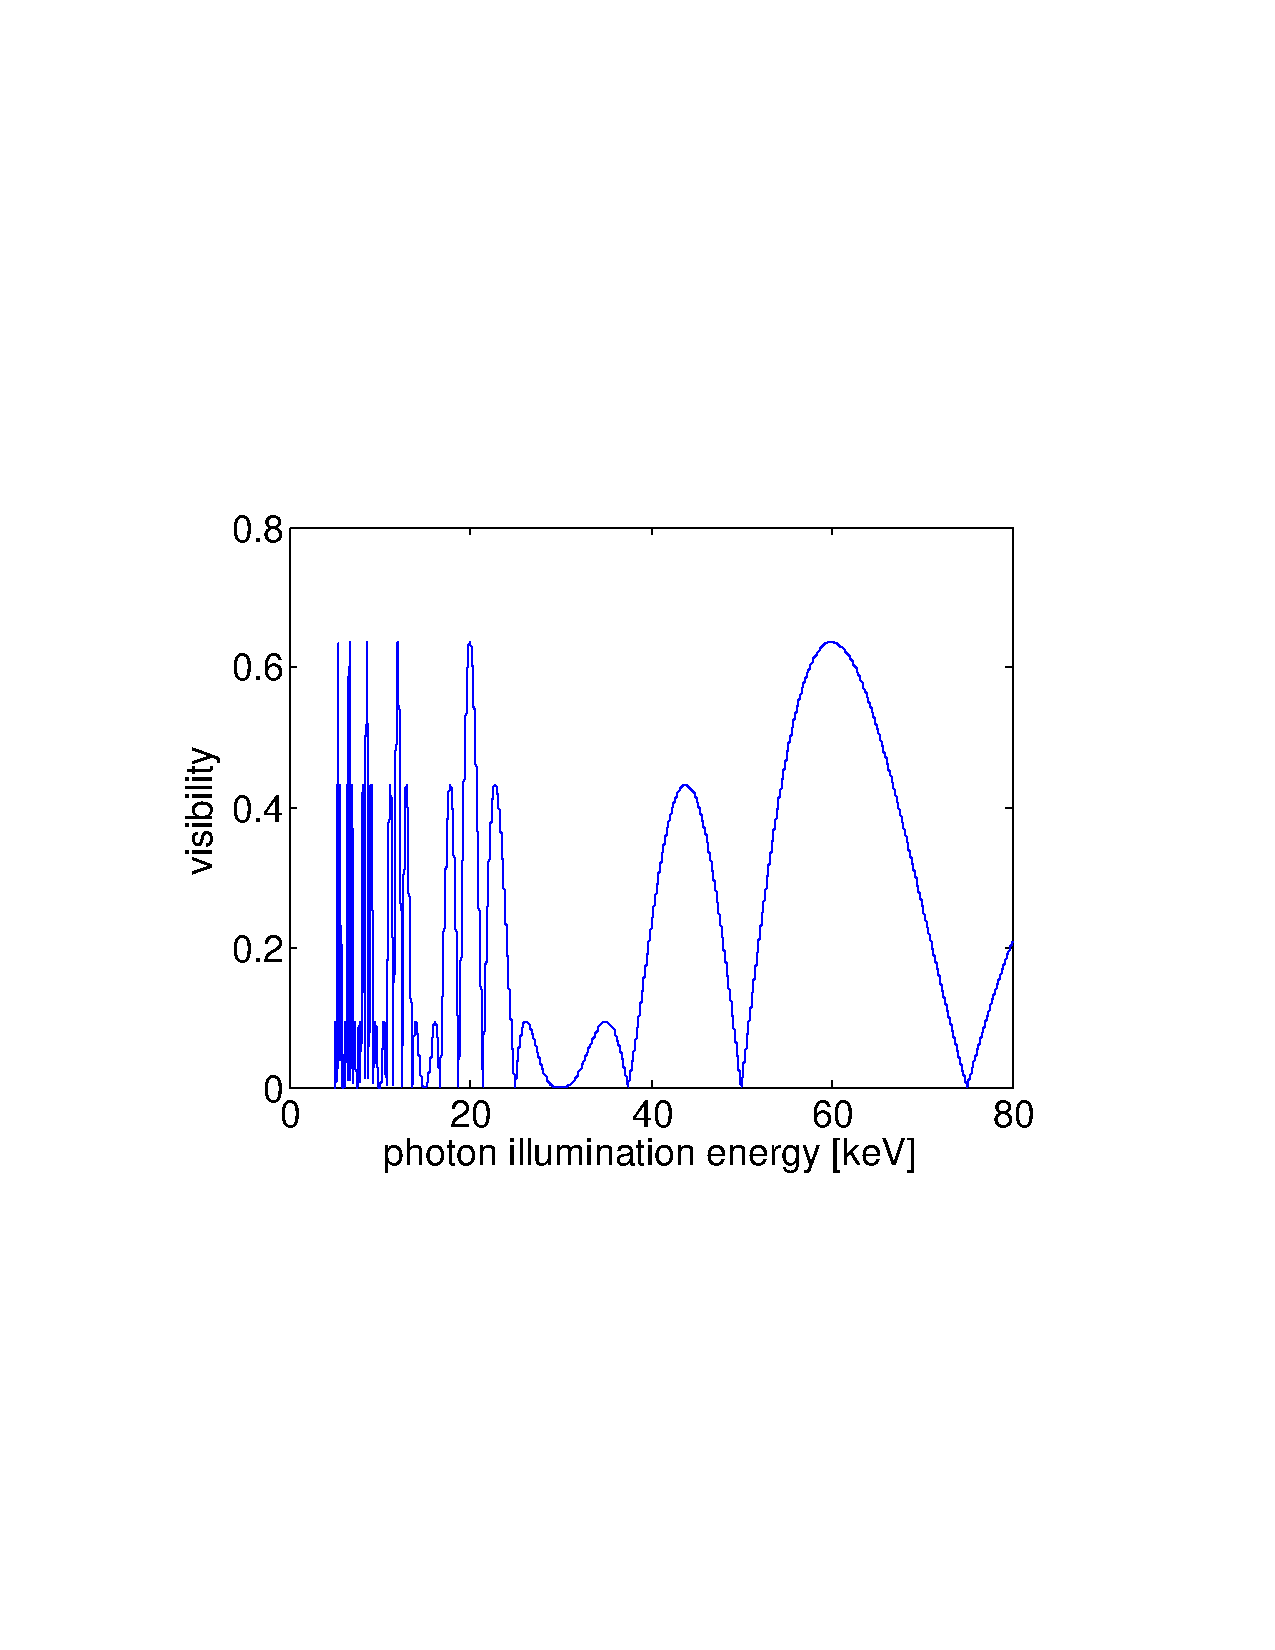
\includegraphics[width=\textwidth]{spectrum_60keV_5TD} 
            \end{subfigure}
        \end{figure}
    \end{frame}

    \begin{frame}
        \frametitle{Single-layer filters}
        transmission $e^{-\mu(\energy) d}$\\
        try different materials.
    \end{frame}

    \begin{frame}
        \frametitle{Multi-layer filters}
        ``Playing'' with the edges.\\
        Many elements $\longrightarrow$ genetic algorithm
        \begin{table}
            \centering
            \begin{tabular}{cc}
                \toprule
                natural selection & X-ray filters\\
                \midrule
                organism & multi-layer filter\\
                gene & thickness of each layer\\
                fitness & flux in the energy window\\
                \bottomrule
            \end{tabular}
        \end{table}
    \end{frame}

    \begin{frame}
        \frametitle{The genetic algorithm}
        At each step (generation), on a population of 50 filters.\\
        running time $< \SI{1}{\second}$ per generation.
        \vspace{\baselineskip}\\
        \begin{enumerate}
            \item evaluate the fitness 
            \item the five \alert{fittest survive} and reproduce
            \item small random \alert{mutations} occur 
        \end{enumerate}
    \end{frame}

    \begin{frame}
        \frametitle{Results of the genetic algorithm}
        \begin{itemize}
            \item fast convergence ($\sim$ 200 generations)
            \item explore many possibilities at once
        \end{itemize}
        \begin{figure}[h]
            \centering
            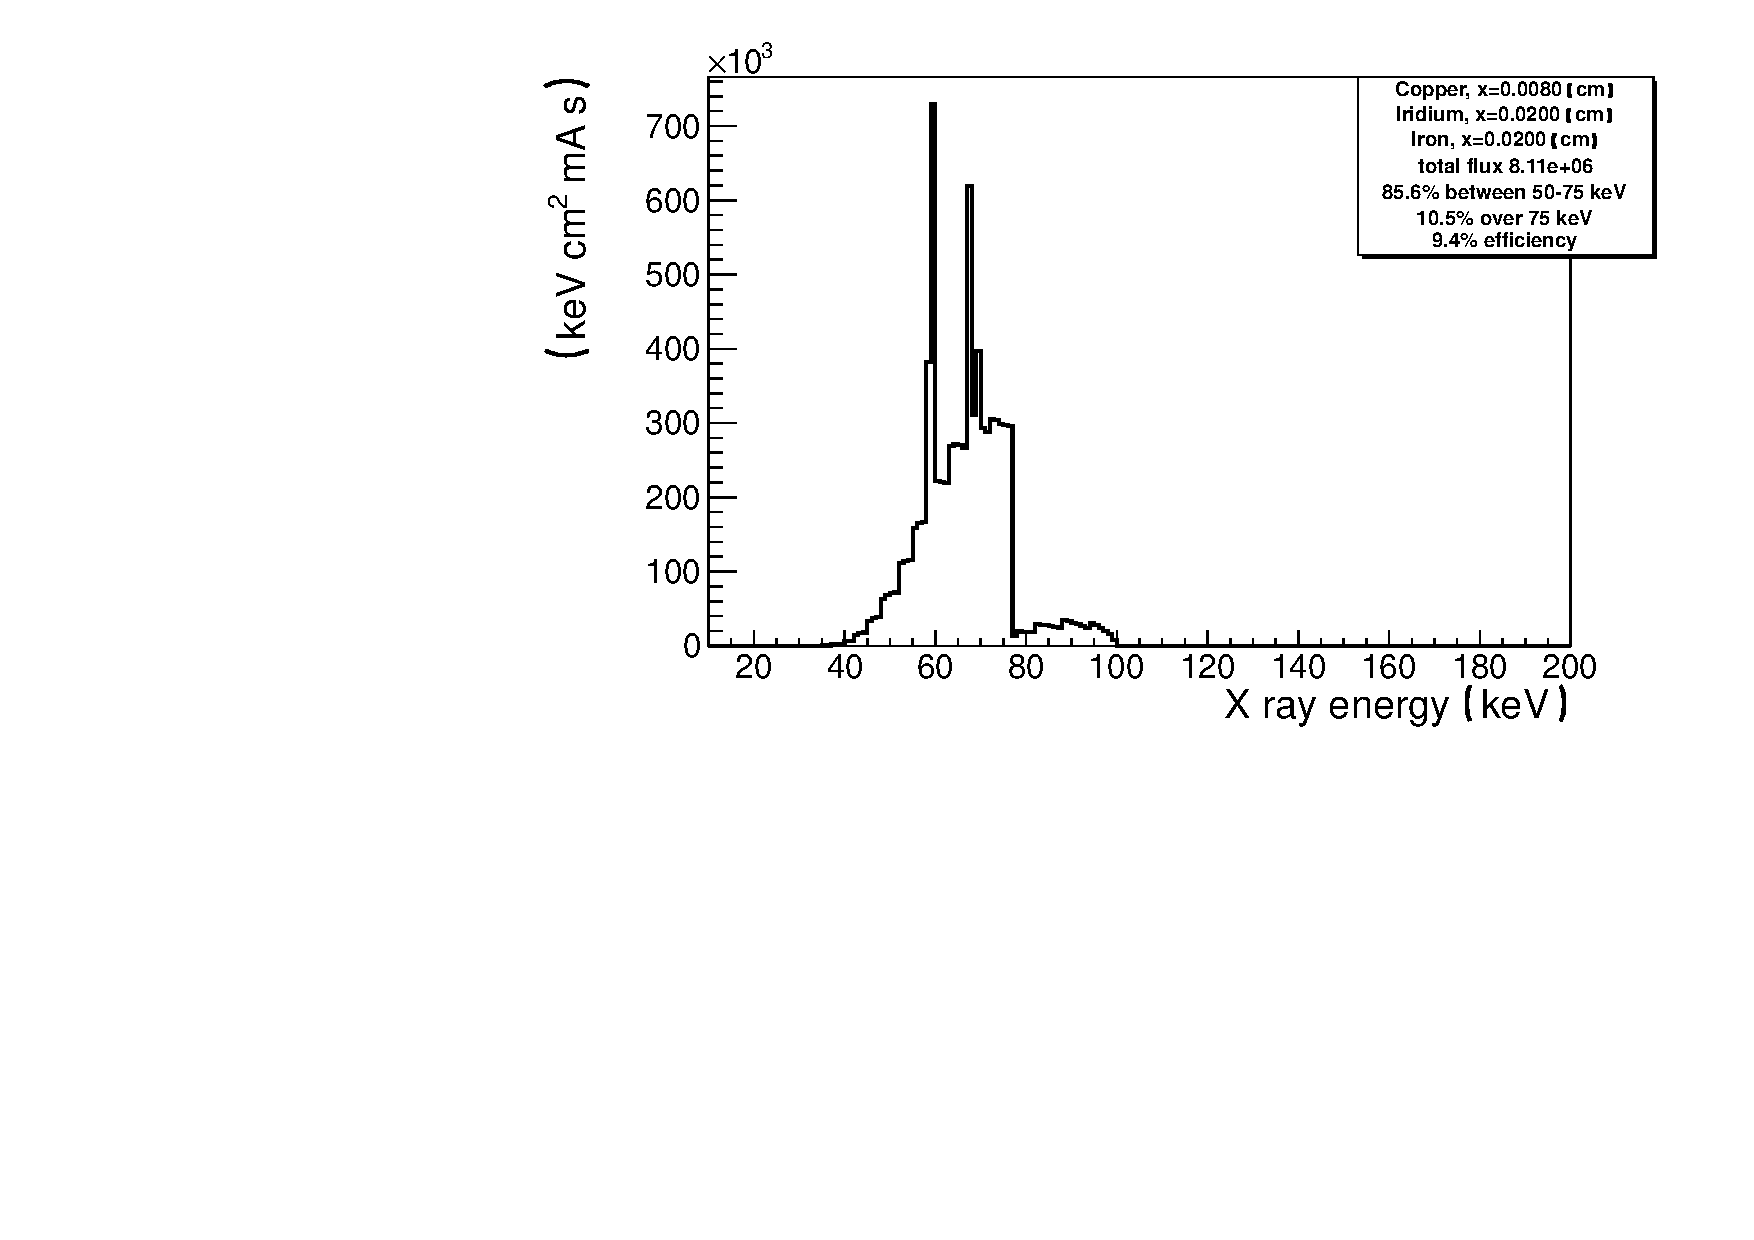
\includegraphics[width=.7\textwidth]{filtered} 
        \end{figure}
    \end{frame}

    \begin{frame}
        \frametitle{Compton scattering}
        cross section increase $\longrightarrow$ noise from large-angle scattering 
        \begin{figure}[h]
            \centering
            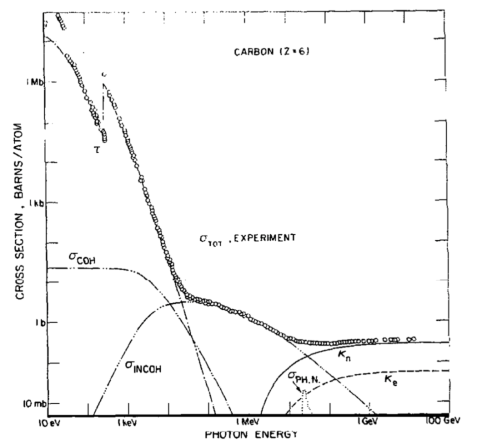
\includegraphics[width=.6\textwidth]{carbon_cross_sections}
        \end{figure}
    \end{frame}

    \begin{frame}
        \frametitle{Compton scattering}
        \begin{itemize}
            \item estimate with Monte Carlo (Silvia\textcopyright)
            \item energy selection as a possible improvement
        \end{itemize}
        \begin{block}
            {}
            High-energy photons scattered at large angles lose a greater
            fraction of their energy with respect to low-energy photons.
            \vspace{.5\baselineskip}\\
            $\Delta \lambda \sim \lambda_{\text{Compton}} = \dfrac{h}{m_e c} =
            \SI{2.4}{\pico\metre}$
            \vspace{.5\baselineskip}\\
            $\lambda(\SI{100}{\kilo\electronvolt}) = \SI{12.4}{\pico\metre}$
            \vspace{.5\baselineskip}\\
            $\dfrac{\Delta \lambda}{\lambda} = \dfrac{\Delta \energy}{\energy} \sim
            \SI{20}{\percent}$
        \end{block}
    \end{frame}

    \begin{frame}
        \frametitle{Silvia's Monte Carlo estimate}
            @\SI{60}{\kilo\electronvolt} $< \SI{1}{\permille}$
        \begin{columns}
            \begin{column}
                {.5\textwidth}
                \begin{figure}[h]
                    \centering
                    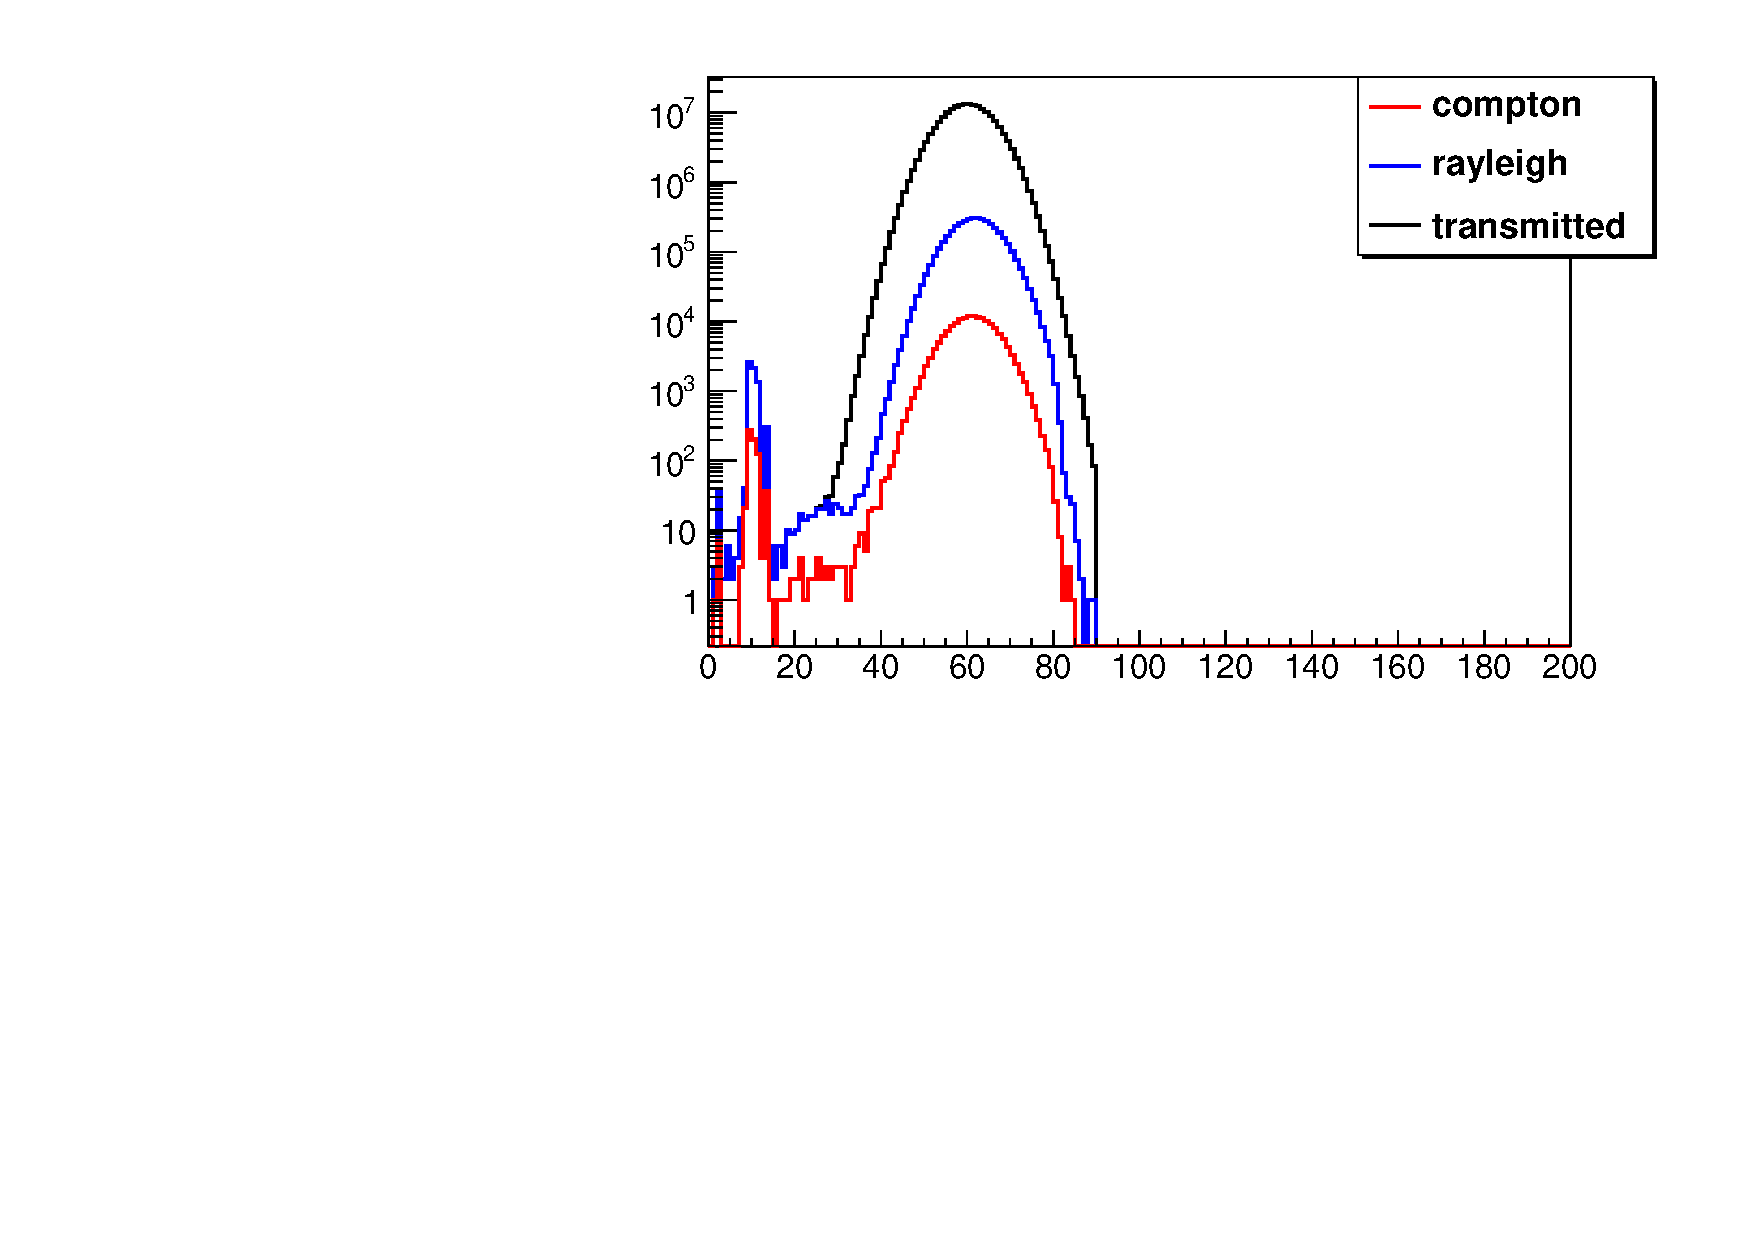
\includegraphics[width=\textwidth]{energy}
                \end{figure}
            \end{column}
            \begin{column}
                {.5\textwidth}
                \begin{figure}[h]
                    \centering
                    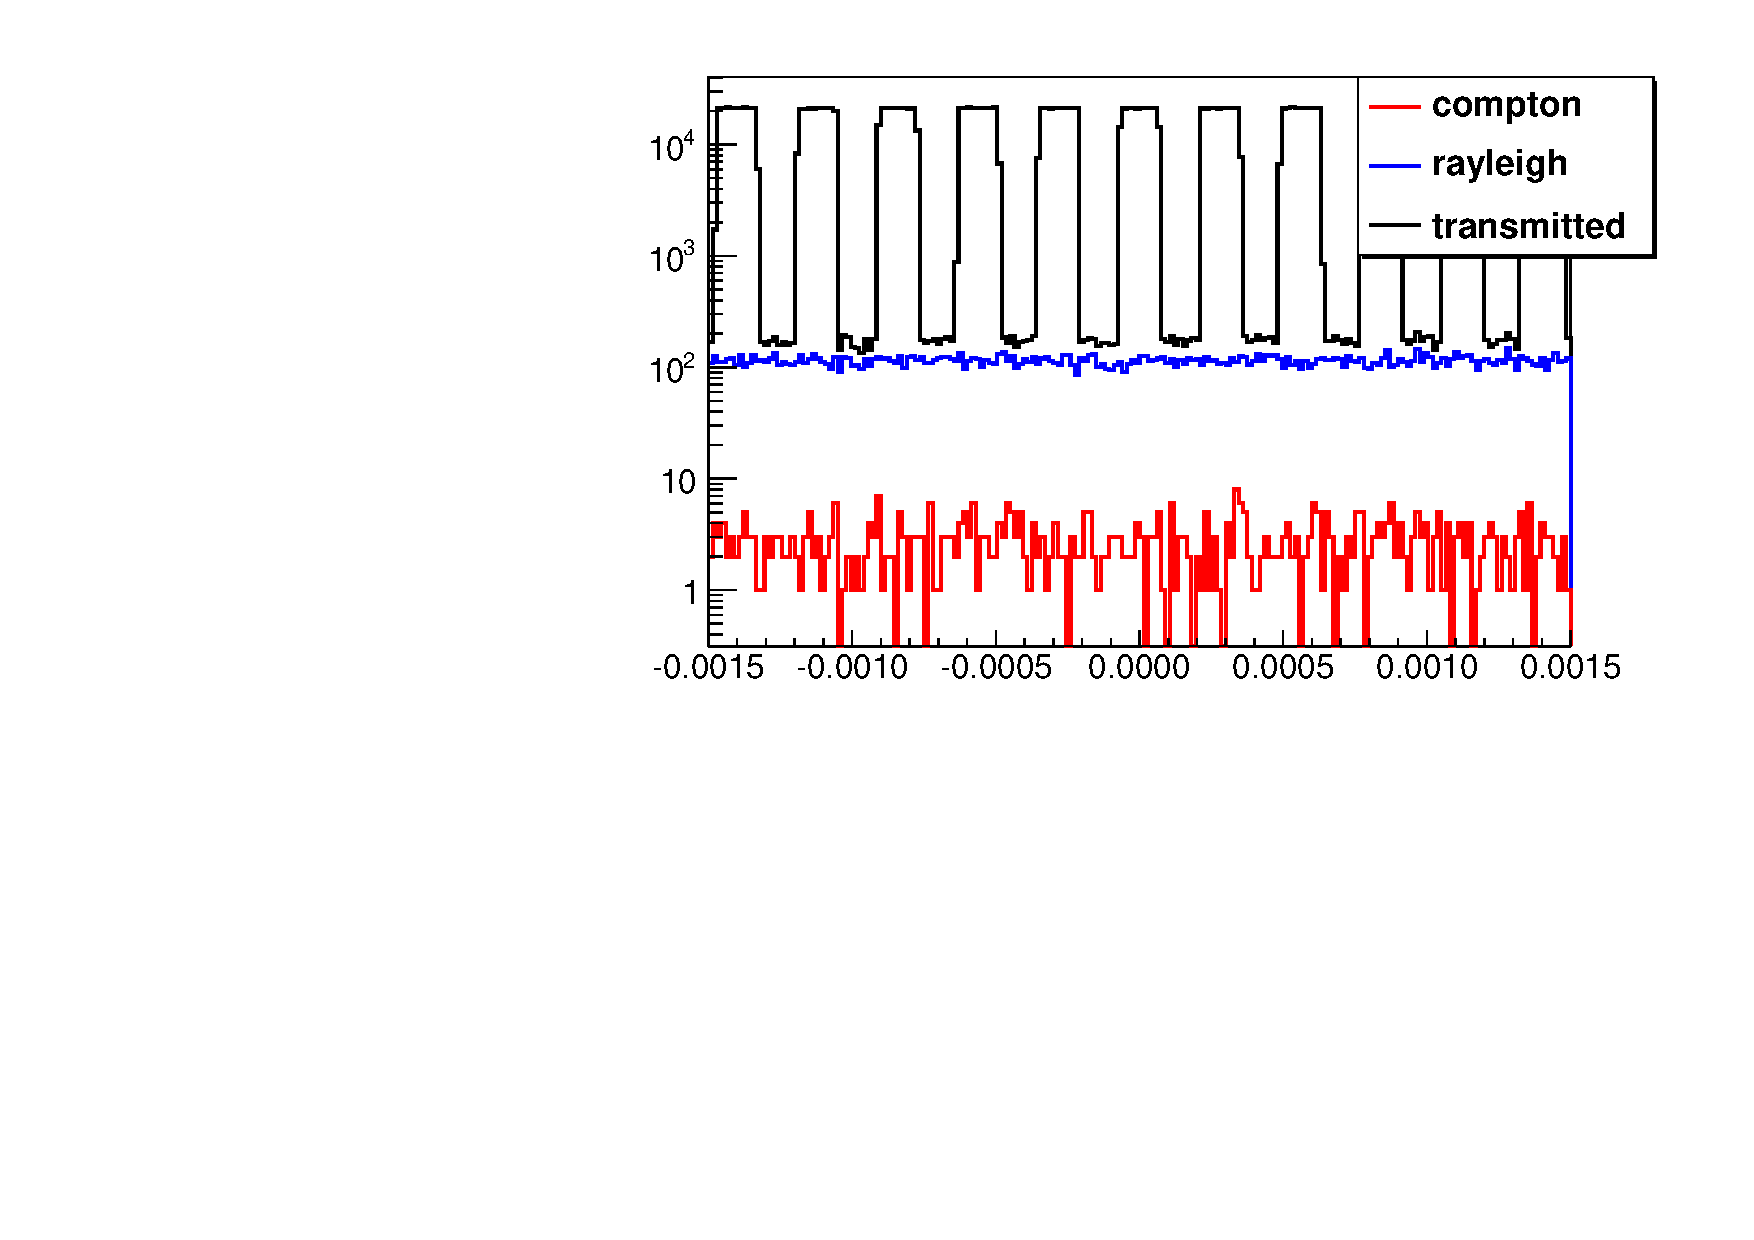
\includegraphics[width=\textwidth]{position}
                \end{figure}
            \end{column}
        \end{columns}
    \end{frame}

    \begin{frame}
        \frametitle{Further ideas for the spectral data}
        \begin{itemize}
            \item absorption and refraction \alert{curves}
            \item enhanced material classification 
            \item student project with Eiger detector (A. Bergamaschi)
        \end{itemize}
        \begin{columns}
            \begin{column}
                {.8\textwidth}
                \begin{figure}[h]
                    \centering
                    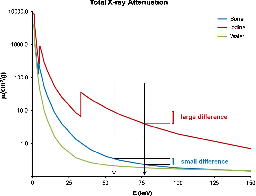
\includegraphics[width=.7\textwidth]{multienergy}
                \end{figure}
            \end{column}
            \begin{column}
                {.3\textwidth}
        \tiny{\emph{Dual- and multi-energy CT: approach to functional imaging},
    Insights Imaging. 2011 April; 2(2): 149–159}
            \end{column}
        \end{columns}
\end{frame}

\begin{frame}
    \frametitle{Thanks Thomas for all the support!}
    And thanks Silvia for the MC simulations!
\end{frame}

\begin{frame}
    \frametitle{Thanks you for your attention!}
    Questions? Comments?
\end{frame}
\end{document}
